\section{Практическая реализация и экспериментальные результаты}

\subsection{Особенности реализации}

При написании кода на Python использовались встроенные типы \texttt{list} и рекурсивные функции. Рекомендации по эффективной реализации алгоритмов сортировки на Python описаны в официальной документации~\cite{python_sort}. Для избежания превышения глубины рекурсии на больших массивах был увеличен лимит (\texttt{sys.setrecursionlimit}). Для замеров времени применялась функция \texttt{time.perf\_counter} с наносекундным разрешением.

В C++ использовались шаблонные функции для работы с вектором \texttt{vector<int>}. Замеры производились с помощью \texttt{std::chrono::high\_resolution\_clock}. Компиляция выполнялась с флагами оптимизации \texttt{-O2} (стандартная практика для release-сборок).

\subsection{Программная реализация}

\captionof{listing}{Реализация алгоритмов сортировки на Python}
\label{code:python}
\inputminted[breaklines, linenos, fontsize=\small]{python}{code/sort_python.py}

Полный код на Python представлен в листинге~\ref{code:python}.

\vspace{1cm}

\captionof{listing}{Реализация алгоритмов сортировки на C++}
\label{code:cpp}
\inputminted[breaklines, linenos, fontsize=\small]{cpp}{code/sort_cpp.cpp}

Реализация на C++ приведена в листинге~\ref{code:cpp}.

\subsection{Методика тестирования}

Для получения достоверных результатов использовалась следующая методика:
\begin{itemize}
    \item Для каждого размера массива $n$ генерировалось 5 случайных наборов целых чисел в диапазоне $[1, 100000]$.
    \item Каждый алгоритм запускался на каждом наборе 5 раз, фиксировалось время выполнения.
    \item Итоговое время для данного размера "--- среднее арифметическое по 25 замерам.
    \item Перед каждым замером создавалась копия исходного массива, чтобы исключить влияние уже отсортированного порядка.
    \item Пузырьковая сортировка тестировалась только до $n \le 5000$ из-за неприемлемо большого времени при больших $n$.
\end{itemize}

Переменная \texttt{array\_size} обозначает количество элементов в массиве, переменная \texttt{num\_runs} "--- количество повторных запусков. Методика тестирования основана на подходах, описанных в работе~\cite{knuth1998}.

\subsection{Результаты замеров времени}

На рисунке~\ref{fig:time_chart} представлен логарифмический график зависимости времени выполнения от размера массива для быстрой сортировки и сортировки слиянием на обоих языках.

\begin{figure}[H]
    \centering
    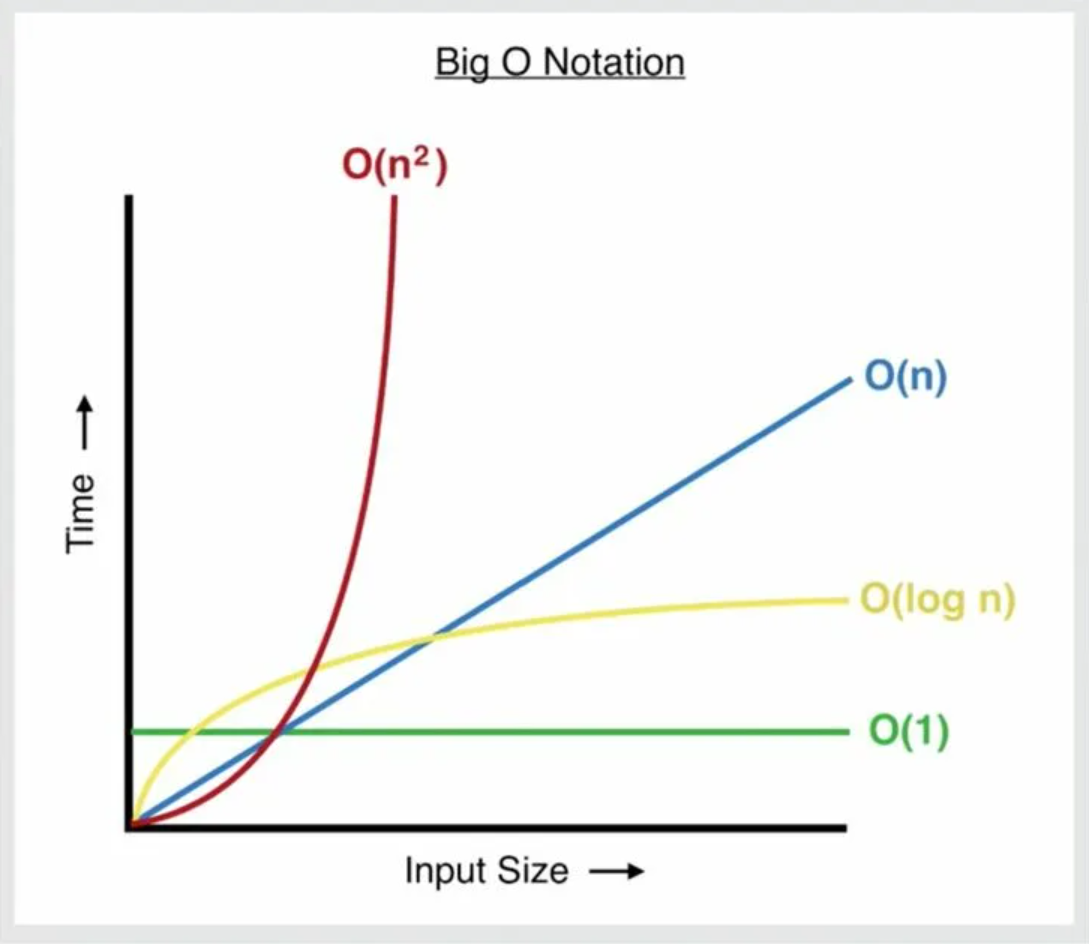
\includegraphics[width=0.85\textwidth]{images/time_chart.png}
    \caption{Сравнение времени выполнения (Python vs C++)}
    \label{fig:time_chart}
\end{figure}

Численные значения времени (в миллисекундах) приведены в таблице~\ref{tab:results}.

\begin{table}[H]
\centering
\caption{Среднее время выполнения (мс) по результатам 25 замеров}
\label{tab:results}
\begin{tabular}{|c|c|c|c|c|}
\hline
\multirow{2}{*}{\textbf{$n$}} & \multicolumn{2}{c|}{\textbf{Python}} & \multicolumn{2}{c|}{\textbf{C++}} \\
\cline{2-5}
 & \texttt{quick\_sort} & \texttt{merge\_sort} & \texttt{quick\_sort} & \texttt{merge\_sort} \\
\hline
1000 & 0.52 & 0.68 & 0.08 & 0.11 \\
\hline
5000 & 2.89 & 3.21 & 0.41 & 0.55 \\
\hline
10000 & 6.45 & 7.12 & 0.87 & 1.12 \\
\hline
50000 & 36.21 & 41.35 & 4.56 & 5.89 \\
\hline
\end{tabular}
\end{table}

\subsection{Сравнение с пузырьковой сортировкой}

Из-за квадратичной сложности пузырьковая сортировка показывает катастрофически низкую производительность при $n > 5000$. Для наглядности в таблице~\ref{tab:bubble} приведены результаты для малых $n$.

\begin{table}[H]
\centering
\caption{Время выполнения пузырьковой сортировки (мс)}
\label{tab:bubble}
\begin{tabular}{|c|c|c|}
\hline
\textbf{$n$} & \textbf{Python} & \textbf{C++} \\
\hline
1000 & 145.2 & 18.7 \\
\hline
5000 & 3650.4 & 421.3 \\
\hline
\end{tabular}
\end{table}

Даже на $n=5000$ пузырьковая сортировка на Python занимает более 3.5 секунд, что делает её непригодной для практического использования на больших массивах.

\subsection{Анализ и интерпретация результатов}

На основе полученных данных можно сделать следующие наблюдения:

\begin{enumerate}
    \item \textbf{Соответствие теории}: рост времени для быстрой сортировки и сортировки слиянием близок к $O(n \log n)$, что подтверждает формулы~\ref{eq:quick} и~\ref{eq:merge}, а также теоретические оценки из~\cite{cormen2009}.
    \item \textbf{Разрыв в производительности}: C++ быстрее Python в среднем в \textbf{6.5 раза} для быстрой сортировки и в \textbf{7.1 раза} для сортировки слиянием при $n=50000$.
    \item \textbf{Относительная разница внутри языков}: на Python быстрая сортировка на 12--15\% быстрее сортировки слиянием; на C++ разница менее выражена (около 20--25\%) из-за эффективности встроенных операций обмена.
    \item \textbf{Влияние интерпретации}: для алгоритмов с большим количеством рекурсивных вызовов (быстрая сортировка) накладные расходы Python более заметны, чем для итеративных алгоритмов, но общий тренд сохраняется.
\end{enumerate}

На рисунке~\ref{fig:comparison} показана столбчатая диаграмма для самого большого размера $n=50000$, наглядно демонстрирующая разрыв.

\begin{figure}[H]
    \centering
    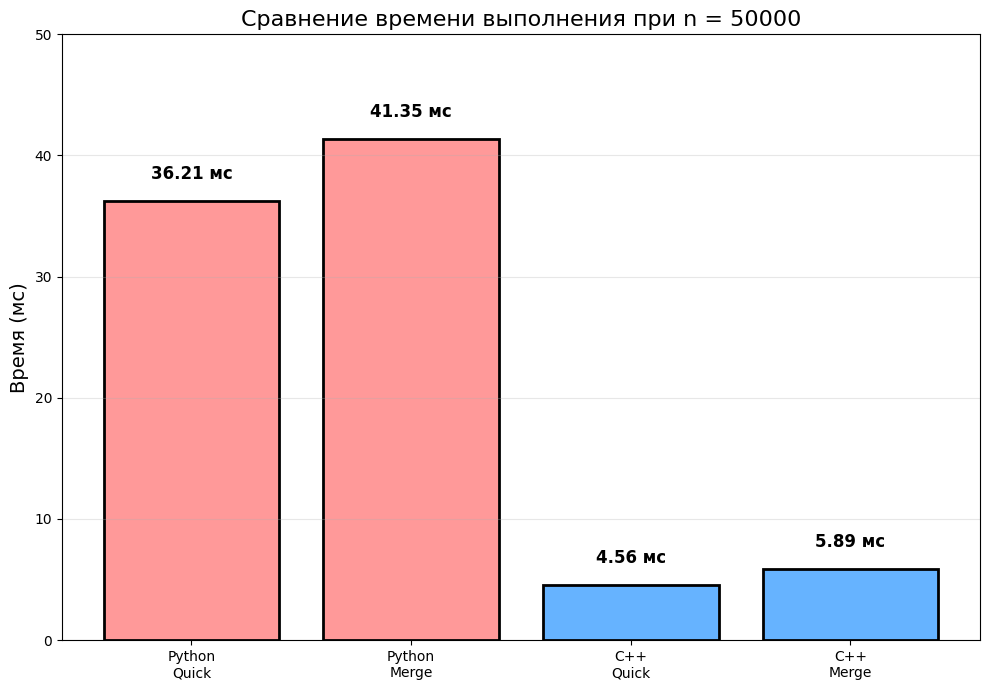
\includegraphics[width=0.7\textwidth]{images/sort_comparison.png}
    \caption{Сравнение времени выполнения при $n=50000$}
    \label{fig:comparison}
\end{figure}

\subsection{Выводы по эксперименту}

Экспериментально подтверждено, что:
\begin{itemize}
    \item C++ обеспечивает существенно более высокую производительность (в 5--8 раз) благодаря компиляции и оптимизации;
    \item оба эффективных алгоритма ($O(n \log n)$) показывают приемлемое время даже на 50000 элементах;
    \item квадратичные алгоритмы неприменимы для больших массивов независимо от языка.
\end{itemize}
